\documentclass{ituthesis}
\usepackage{hyperref}
\usepackage[]{float} 
\usepackage[]{csquotes} 

\settitle{The Practical Guide to Levitation}
\setauthor{Ahmad Salim Al-Sibahi}
\setsupervisor{Dr. Peter Sestoft}
\setextrasupervisor{David R. Christiansen}
\setdate{September 1, 2014}

\begin{document}
%\selectlanguage{danish}

\frontmatter

\thetitlepage
\newpage

\chapter*{Abstract}
Goal: Implementation of levitation in a realistic setting, with practical performance benefits.
\blockquote{DISCLAIMER: This is a draft and as such is incomplete, incorrect and can contain grammatical errors.
Although I claim originality of this report, many underlying ideas are based on current work in the scientific community which will be correctly attributed
when the work is complete.}

\cleardoublepage
\setcounter{tocdepth}{1}
\tableofcontents

\mainmatter

%from memoir documentation:
%TeX tries very hard to keep text lines justified while keeping the interword spacing as constant as possible, but sometimes fails and complains about an overfull hbox.
%The default mode for LaTeX typesetting is \fussy where the (variation of) interword spacing in justified text is kept to a minimum. Following the \sloppy declaration there may be a much looser setting of justified text.
%Additionally the class provides the \midsloppy declaration which allows a setting somewhere between \fussy and \sloppy.
%fewer overfull lines than \fussy, and fewer obvious large interword spacing than with \sloppy.
%the memoir manual also uses \midsloppy!
\midsloppy
% try harder to avoid widows and orphans
\sloppybottom

\chapter{Introduction}
\label{cha:Intoduction}
\section{Context}
\label{sec:Context}
Algebraic datatypes such as booleans, lists or tree form a core part of modern functional programming.
While most functions work directly on such datatypes, sometimes it is the case that the function we write are purely repetitive such as those for structural equality or pretty printing.
In fact it seems that it is possible to write a function over the structure of the datatype definition which the computer could use to derive actual function for particular datatypes.

Enter the world of \textit{generic programming} where the target data is the datatype describing the structure of other datatypes which is often called the \textit{description}.
While generic programming sounds promising, there has usually been issues regarding usability in traditional functional languages. To represent the description it is often required to use special language extensions, and the programming style is almost
orthogonal to ordinary programs.

In dependently-typed languages such as Idris or Agda however, it seems that it possible to mitigate such issues.
Due to the nature of dependently-typed languages it is possible to create a correct description using ordinary datatype definitions.
Furthermore, Chapman et al. present in `The Gentle Art of Levitation' how it is possible to build a self-supporting type system which is able to synthesise descriptions to ordinary types and is still powerful enough to describe the description datatype itself.
Therefore, generic programming is not different from ordinary programming in such system.

\subsection{The Importance of Genericity in Dependently-typed Languages}
\label{sub:TheImportanceofGenericityinDependently-typedLanguages}
\textit{The similarity of structure and various slightly-different indexing of types.}


\section{Problem Definition}
\label{sec:ProblemDefinition}
The current work on generic programming in dependently-typed languages presents both elegant and correct ways to represent the structural descriptions of datatypes. Furthermore, it allows the programmer to save both time and boilerplate code by using generic programming based on ordinary programming techniques.

Yet in many ways, the state of the art has been mostly theoretically oriented which can lead to some issues when described types are to be used in a practical manner.
First of all, multiple incompatible descriptions are presented in the current field and often even in the same paper, which is not particularly attractive in a practical setting.
Secondly, there has been little work on how to integrate such descriptions in languages which contain features such as type classes and proof scripts.
Finally, datatypes synthesised from descriptions create large canonical terms and as such both type checking and runtime performance is very slow.
In summary, if an efficient and easily usable version of described types could be implemented successfully it would save programmers both time and effort in writing repetitive functions without any large performance penalties.

\section{Aim and Scope}
\label{sec:AimandScope}
The main aim of this research is to provide a practical and efficient implementation of described types in Idris.

One key part is therefore to find a good definition of the description that supports many common datatypes.
I seek to mainly base my effort on reusing some of the existing work on descriptions, and not try to improve underlying type theory to support inductive-inductive and inductive-recursive datastypes; neither will I focus on supporting all language features of Idris such as implicit arguments and codata definitions.
Another key part is to present realistic examples using generic functions by implementing a mechanism for type class deriving and a Scrap Your Boilerplate library for generic querying and traversal.
In the end, I seek to use partial evaluation to optimise the generic functions with regards to specific descriptions to achieve near hand-written performance metrics. %Elaborate when I know more about PE\ldots

\section{Significance}
\label{sec:Significance}
The main contributions of my research are:

\begin{itemize}
  \item an example-based tutorial for understanding described types in the context of a practical programming language, namely Idris
  \item an generic implementation of common operations such as decidable equality, pretty printing and functors, which can be used to provide default implementations to type class methods.
  \item a discussion of challenges that arise when trying to implement a SYB-style generics library in dependently typed languages
  \item optimisation techniques based on partial evaluation for reducing runtime size and time overhead for described types and accompanying generic functions
  \item metrics that show how generic programming using described types is a viable option to reduce boiler-plate without significant cost in performance
\end{itemize}
\section{Overview}
\label{sec:Overview}
I will present the report as follows. In Chapter~\ref{cha:GenericProgramming}, I will present an introduction to described types specifically focusing on recent developments using dependently-typed programming languages.
In Chapter~\ref{cha:PartialEvaluation}, I will present an overview of techniques for partial evaluation of functions and specialisation of datatypes. In Chapter~\ref{cha:LevitatingIdris}, I will discuss specifically how described types are implemented in Idris and I will continue with the practical examples in Chapter~\ref{cha:PracticalExamples}.
In Chapter~\ref{cha:OptimizingIdrisforFlight} I will present what optimisations were made in order to improve the runtime performance of described types and generic functions. I will evaluate the results in Chapter~\ref{cha:Evaluation}, comparing the performance of generic implementations to hand-written ones.
Finally, I will discuss what challenges still lie ahead and conclude in Chapter~\ref{cha:Discussion}.
\chapter{Generic Programming}
\label{cha:GenericProgramming}
\section{The Generic Structure of Inductive Data Types}
\label{sec:TheGenericStructureofInductiveDataTypes}
\subsection{Anatomy of a Datatype}
\label{sub:AnatomyofaDatatype}
In order to understand how a description might look like, let us first start by looking closely at how datatypes are structured. In Figure~\ref{fig:anatomydatatype}, I present an annotated version of a typical dependently-typed datatype that represents vectors.

\begin{figure}[ht]
\begin{center}
    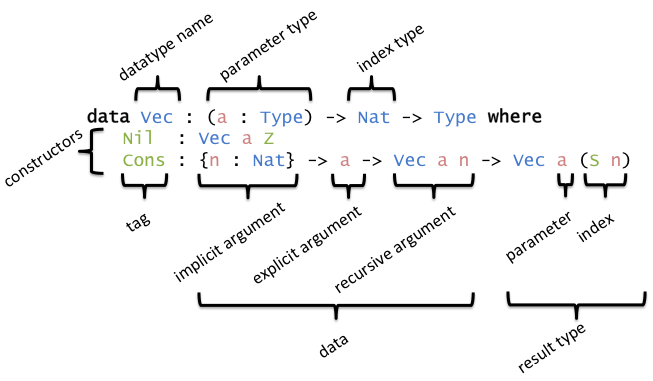
\includegraphics[scale=0.5]{Figures/AnatomyOfADatatype.png}
\end{center}
\caption{Annotated Components of a Datatype Declaration}
\label{fig:anatomydatatype}
\end{figure}

A datatype consists of a type constructor which describes what type-level arguments are required, and zero or more data constructors which describe how to create values of the datatype.
The type constructor consists of three components: a name for the datatype, types of any possible parameters, and the types of possible indices. In Figure~\ref{fig:anatomydatatype} is no difference between a parameter type or an index type due to the fact that
Idris can figure this out automatically. \footnote{If the argument to a type constructor doesn't change in the data constructor declarations Idris considers that a parameter, and otherwise an index.}

Similarly to the type constructor, data constructors also need names, also called \textit{tags}.
Following the tag, the data constructor declaration contains the types of the arguments stored in the constructor and resulting type which must use the type constructor of the data type.
In our example two constructors are declared, \texttt{Nil} and \texttt{Cons}.
\texttt{Nil} doesn't hold any data, so it only needs to define the resulting type which is \texttt{Vect a Z} (a vector with length 0).
\texttt{Cons} contains three different types of arguments: an ordinary implicit argument, an ordinary explicit argument, and an explicit argument to the type itself (recursive); the resulting type for \texttt{Cons} is \texttt{Vect a (S n)} (i.e. a vector of length 1+n where n is the length of the recursive argument).

\subsection{A Description for Datatypes}
\label{sub:ADescriptionforDatatypes}
It is now possible to try to represent a suitable description datatype. Figure~\ref{fig:descriptiondatatype} presents one possible solution, influenced mainly by the work of McBride and Diehl.

\begin{figure}[ht]
\begin{center}
    \includegraphics[scale=0.5]{Figures/ADescriptionforDatatypes.png}
\end{center}
\caption{Datatype for describing other datatypes}
\label{fig:descriptiondatatype}
\end{figure}

In order to allow datatypes to be indexed by values of various types, the description structure takes a parameter that describes what the type of indices must be.
Additionally, the description has three constructors:
\begin{itemize}
  \item  \texttt{Ret} represents the end of a description and takes as argument what value the index of the resulting type must be
  \item  \texttt{Arg} represents the addition of an argument of any type to a given description; the first argument of \texttt{Arg} is the type of argument expected and the second argument is the rest of the description dependent on a value of that type.
  \item  \texttt{Rec} represents a recursive argument of the described datatype and take two arguments: the index of the recursive instance of the datatype and the rest of the description.
\end{itemize}

\begin{figure}[ht]
\begin{center}
    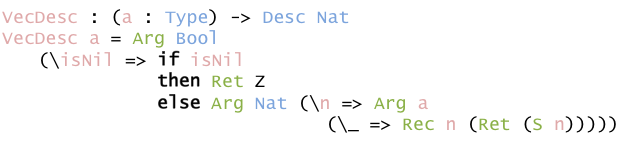
\includegraphics[scale=0.5]{Figures/VectorDescription.png}
\end{center}
\caption{Described version of Vec}
\label{fig:descvec}
\end{figure}

The astute reader might have some questions at this point such as: how is it possible to choose between different constructors? where do parameters go in the description? and why is there only one type for indicies?
I will now try to answer these questions using Figure~\ref{fig:descvec}.

One step towards building a value that describes a particular datatype is defining its type signature
including what types the parameters and indices of the finished datatype are. In our example of Figure~\ref{fig:descvec},
the parameter is specified to be given as an argument to the description value and is not represented internally as such in the final description i.e., it is not possible
to distinguish a parameter from other values when the final description is constructed.
Contrary to parameters, the type of indices must be specified as an internal part of the description in order to ensure that indices specified by recursive arguments match in the final description.
Since \texttt{Desc} only takes one argument for specifying the types of indices more demanding datatypes will need to collect multiple indices into one dependent pair, e.g.,
a datatype with signature \texttt{(n : Nat) -> Fin n -> Type} must use the dependent pair \texttt{(n : Nat ** Fin n)} as type of index.

Another step required for describing a datatype is defining how to choose a particular constructor.
A solution could be the one presented in Figure~\ref{fig:descvec} where a boolean argument \texttt{isNil} is used to decide whether the resulting description should be for the \texttt{Nil} or \texttt{Cons} constructors.
However, since this solutions is fairly primitive and doesn't capture information such as constructor tags, a better but more complex encoding will be presented in Section~\ref{sub:AnInformativeEncodingofConstructors}.

Finally, the constructors themselves must be described.
\texttt{Nil} doesn't contain any data so we simply use \texttt{Ret Z} which indicates that the description is finished and the resulting type is expected to have index \texttt{Z}, analogously to Figure~\ref{fig:anatomydatatype}.
\texttt{Cons} takes first two ordinary arguments: a \texttt{Nat} argument\footnote{Implicit arguments is a feature of Idris that only works on top-level declarations and as such are all specified explicitly in the description.} to be used for the necessary indices, and an argument of the parameter \texttt{a}. Following these arguments we take a recursive argument specified using \texttt{Rec} that must satisfy to have the value of the input \texttt{Nat} argument \texttt{n} as index, i.e. the argument must be of type \texttt{Vect a n}. We finish the description with \texttt{Ret} and specify that the resulting index must be \texttt{S n} as expected.

\subsection{An Informative Encoding of Constructors}
\label{sub:AnInformativeEncodingofConstructors}
In Section~\ref{sub:ADescriptionforDatatypes} I had presented the choice of constructors using a boolean variable and concluded that it was both primitive and had lacked
necessary information such as the tag of a particular constructor. I will in this section present a more informative encoding of constructors, and show how it is possible to use that encoding when describing datatypes.

\section{The (Mostly) Gentle Art of Levitation}
\label{sec:TheMostlyGentleArtofLevitation}
\textit{The elegance of a complete theorem for both ordinary and generic programming. Highlighting of possible issues with performance.}

\chapter{Partial Evaluation}
\label{cha:PartialEvaluation}

\section{Functions and Constant Inputs}
\label{sec:FunctionsandConstantInputs}
\textit{General introduction about partial evaluation.}

\section{Binding-time Analyses of Programs}
\label{sec:Binding-timeAnalysisofPrograms}
\textit{Finding the relevant constant parts of the program.}

\section{Specialisation as a Form of Optimization}
\label{sec:SpecialisationasaFormofOptimization}
\textit{Performance benefits of program specialisation. Pitfalls.}

\chapter{Levitating Idris}
\label{cha:LevitatingIdris}

\section{A Pragmatic Implementation of Levitation}
\label{sec:APragmaticImplementationofLevitation}
\textit{How the general concept of levitation was transferred to Idris.}

\section{Description Synthesis from Ordinary Data Declarations}
\label{sec:DescriptionSynthesisFromOrdinaryDataDeclarations}
\textit{How ordinary data-declarations are synthesized to levitational descriptions.}

\chapter{Practical Examples}
\label{cha:PracticalExamples}

\section{Generic Deriving}
\label{sec:GenericDeriving}
\textit{Examples of generic deriving of algorithms like decidable equality, pretty printing and possibly eliminators via generic structure.}

\section{Uniplate for Idris}
\label{sec:UniplateforIdris}
\textit{A version of the Uniplate library for Idris based on} \url{http://community.haskell.org/~ndm/uniplate/} \textit{and} \url{http://www-ps.informatik.uni-kiel.de/~sebf/projects/traversal.html} \textit{.
This is useful for traversing structures in a generic fashion and especially when dealing with small changes in large data structures (such as compiler ADTs)}

\chapter{Optimizing Idris for Flight}
\label{cha:OptimizingIdrisforFlight}

\section{Specialising Constructors for Specific Types}
\label{sec:SpecialisingConstructorsforSpecificTypes}
\textit{How generalized constructors of described types, are specialised as ordinary data structures.}

\section{Online Erasure of Unused Arguments}
\label{sec:OnlineErasureofUnusedArguments}
\textit{How some type infromation is to be erased at compile time to reduce elaboration overhead. Very hypothetical.}

\section{Static Initialization of Generic Functions}
\label{sec:StaticInitializationofGenericFunctions}
\textit{How algorithms that are dependent on the generic structure of a datatype are optimized. Discuss benefits of having a JIT/Profiling information for future work.}

\chapter{Evaluation}
\label{cha:Evaluation}

\chapter{Discussion}
\label{cha:Discussion}

\section{Future Work}
\label{sec:FutureWork}

\section{Conclusion}
\label{sec:Conclusion}

\end{document}
